Έγινε εκτέλεση των δύο υλοποιήσεων στα web graphs των \textcite{snapnets}.

Παρακάτω παρουσιάζονται διαγράμματα τα διάφορα χαρακτηριστικά των εκτελέσεων.
\begin{center}
\begin{figure}
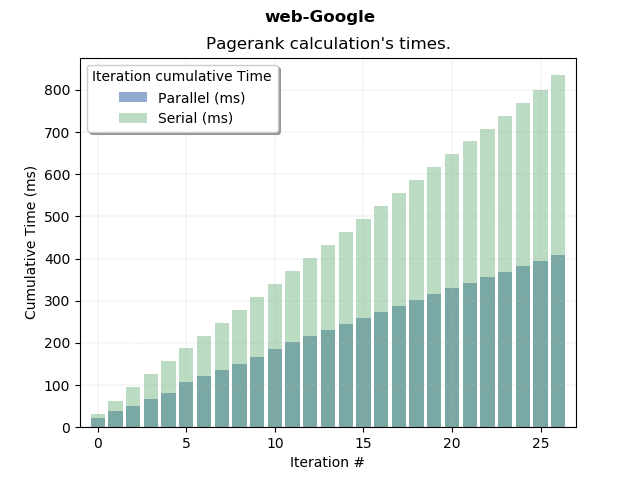
\includegraphics[width=\linewidth]{plots/it_time.png}
\caption{Χρονική εξέλιξη των δύο υλοποιήσεων. 4-πύρηνο σύστημα.}
\end{figure}

\begin{figure}
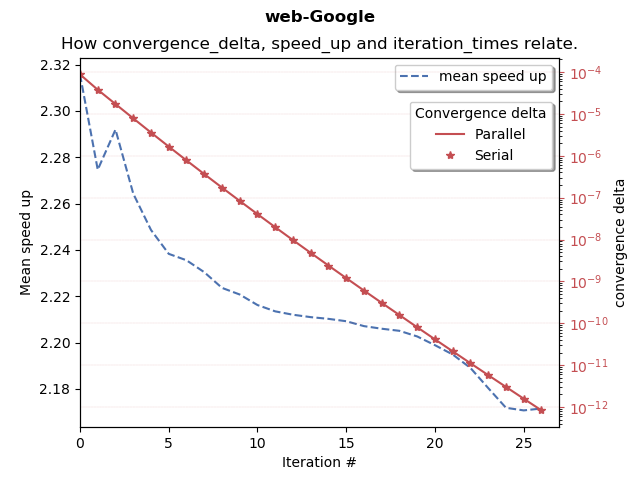
\includegraphics[width=\linewidth]{plots/speed_up.png}
\caption{Σχέση σταθεράς σύγκλισης, επιτάχυνσης και αριθμού επαναλήψεων. 4-πύρηνο σύστημα.}
\end{figure}

\begin{figure}
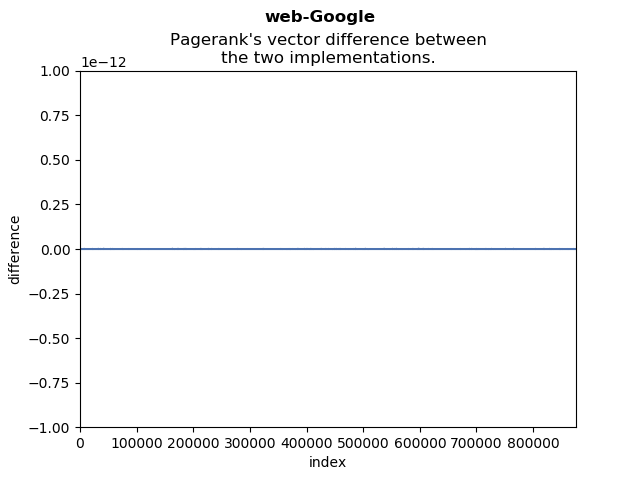
\includegraphics[width=\linewidth]{plots/diff.png}
\caption{Διαφορά των δύο υλοποιήσεων στο τελικό διάνυσμα.}
\end{figure}

\begin{figure}
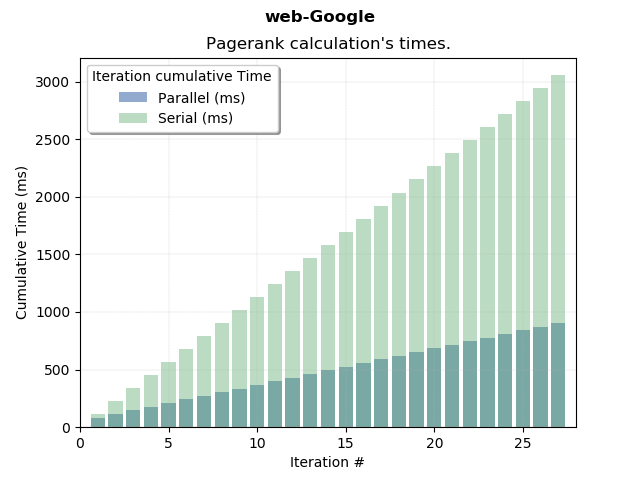
\includegraphics[width=\linewidth]{plots/it_times_diades.png}
\caption{Χρονική εξέλιξη των δύο υλοποιήσεων. 8-πύρηνο σύστημα.}
\end{figure}

\begin{figure}
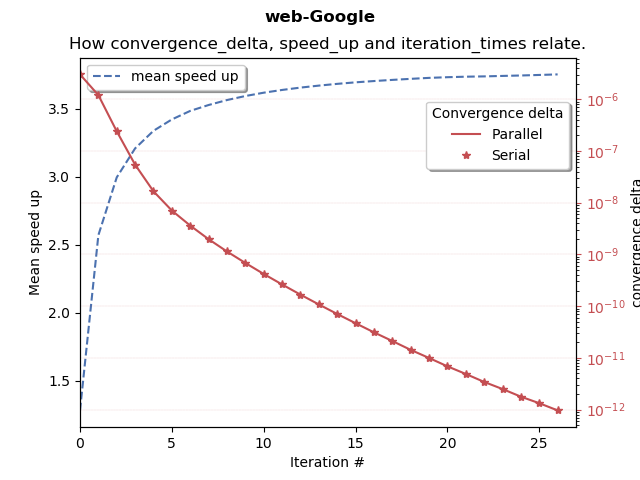
\includegraphics[width=\linewidth]{plots/speed_up_diades.png}
\caption{Σχέση σταθεράς σύγκλισης, επιτάχυνσης και αριθμού επαναλήψεων. 8-πύρηνο σύστημα.}
\end{figure}

\begin{figure}
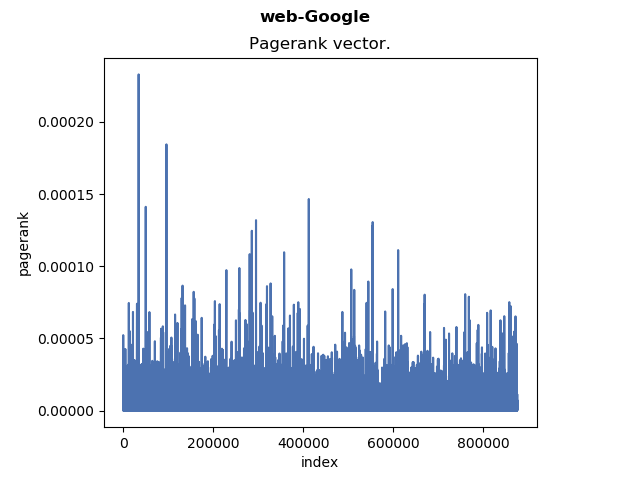
\includegraphics[width=\linewidth]{plots/pagerank.png}
\caption{Το αποτέλεσμα για κάθε κόμβο.}
\end{figure}

\end{center}
Τα web graph που χρησιμοποιήθηκε περιείχε 875.713 κόμβους με 4.563.235 συνδέσμους ενώ δύο συστήματα έχουν τα εξής χαρακτηριστικά: 
\begin{enumerate}

\item 4 πύρηνο σύστημα
\begin{itemize}
\item Intel(R) Core(TM) i5-4670 CPU @ 3.40GHz.
\item 8GB DDR3 RAM
\item gcc version 7.3.0
\end{itemize}

\item 8 πύρηνο σύστημα (diades)
\begin{itemize}
\item Intel(R) Xeon(R) CPU E5420  @ 2.50GHz.
\item 8GB DDR3 RAM
\item gcc version 5.4.0
\end{itemize}
\end{enumerate}

Στα παραδοτέα, περιέχονται έτοιμα τα αποτελέσματα και για τα υπόλοιπα web-graphs. Γενικώς, παρατηρήθηκε ικανοποιητική επιτάχυνση με ταχύτητες έως και 240\% στο τετραπύρηνο ή/και έως 360\% στο οχταπύρηνο σύστημα σε σχέση με τη σειριακή υλοποίηση, για όλα τα δεδομένα με εξαίρεση το web-BerkStan graph όπου ο edge-coloring αλγόριθμος δημιούργησε ιδιαίτερα αυξημένο αριθμό ομάδων. Σε εκείνη την περίπτωση, ο πιο σύγχρονος και γρήγορος επεξεργαστής του 4-πύρηνου συστήματος, εμφάνισε επιτάχυνση έως 120\% περίπου.

Στην παράλληλη υλοποίηση δίνεται και η δυνατότητα επιλογής σταθερού αριθμού threads που θα δημιουργήσει το openMP, η επιλογή αυτή, όμως, οδηγεί συνήθως σε χειρότερη επίδοση του προγράμματος.


